% 来源：OEBPS/Text/Section0001_split_003.xhtml#sigil_toc_id_27

\BookChapter{17}
\section[第17章\q 加速财富积累第1招：储蓄更多，投资更多]{第17章\\ 加速财富积累第1招：储蓄更多，投资更多}

\begin{BookQuote}
好像每件事都在你的掌控之中，那就意味着你跑得不够快。

\hfill ——马里奥·安德列蒂
\end{BookQuote}

祝贺你，你已经朝着财务自由迈出了一大步！大多数人并没有花时间去考虑他们的整体财务状况，创建一个规划；只有少数人这样做了，这非常不容易，这个过程会激起你各种各样的情绪。很强烈，很吓人。我当初也做了财务规划，激起了内心各种各样激烈的情绪，所以我能理解你的感受。但是现在你已经完成你的财务规划了，给自己一点时间好好享受一下你的胜利。问问自己，你看了自己的财务规划的真实感受是什么？你是不是对你和你家庭的未来财务状况感觉挺乐观？你是不是很兴奋，因为你发现你的财务梦想比原来想象的实现时间要近多了？还是你一想到它就很害怕，因为你一看到这个财务规划，就觉得自己可能永远无法实现财务梦想了？你是不是深陷于债务之中，开始怀疑你能不能从这个金钱深坑中挖出一条生路？

不管你现在的财务状况如何，到了什么样的地步，这都没有关系。你已经跨出了好几大步，现在根本不可能掉头回去了。打个比方，现在你已经学会如何走了，那么接下来让我教你如何跑。接下来的几章，要让你好好想想如何让你的财务梦想更快地实现，比你想象到的速度还要快。拥有远大的梦想，并用行动让梦想成真，然后想办法加快梦想成真的速度。你是不是也曾有过非常忙乱的一天，不停地和时间赛跑，克服重重困难，终于提前完成了任务？你可以提前下班了，相当于又额外争取回来一两个小时的生活时间，这绝对是份礼物——这份奖赏让你觉得整个世界都站在你这边支持你。你可以去健身房跑跑步，或者出去找朋友喝杯酒，或者飞快地跑回家去抱抱亲爱的小宝贝——能哄孩子上床睡觉感觉好幸福。

我经常密集地出差旅行，密集得让我发疯。我在不同的国家，不同的大洲，穿越不同的时区，在全世界到处飞来飞去，就像一个环球旅行观光客一样飞个不停，但我只有旅行，没有观光，忙的都是业务。如果我去某个地方的到达时间提前了，如果我一周能额外空出一些时间，再次集中精神，或者陪陪老婆、孩子，我就会充满能量，兴奋激动。因为我找到了一些多出来的时间。

如果多出来的时间不只是一两个小时，事情又会怎么样？如果你能找到的空闲时间，并不只是多出来的一两个小时，而是从财务上讲，多出来需要积蓄2年的财富，或者多出了需要5年积蓄的财富呢？甚至多出来需要10年积蓄的财富，让你享有充分的自由，不用再去靠工作赚钱养家，以维持你现在的生活方式呢？这正是下面这些内容承诺做到的事情。即使你现在的规划看起来不太可能让你达到你梦想的财富水平，这些内容也可以展示给你如何改变你的规划，为你的生命打开新的机会之门——额外的钱，额外的时间，以及终极的自由。

\begin{BookQuote}
得到了时间，就得到了一切。

\hfill ——本杰明·迪斯雷利
\end{BookQuote}

如果你正在加速计划实施，那么你有五个核心的策略。你可以只用其中一招或者五招齐用——这完全由你决定。其中任何一招都能显著地加快你的财富积累的速度，让你更快地实现自己的财务梦想：财务安全，财务独立，财务自由。数招并用，没有人能阻挡你飞一般地前进。

\begin{BookQuote}
你要致富，有两条路可选，一条路是拥有的多而需要的少，另一条路是需要的少而拥有的多。

\hfill ——吉姆·莫特
\end{BookQuote}

\subsection{储蓄更多，投资更多}

你加速自己计划实施的第一个方法是储蓄更多，用这些储蓄来投资，获得复利增长。我知道，这并不是你想看到的。也许你甚至想说：“托尼，我的每一分钱都得花掉，我根本不可能储蓄更多，无论在什么情况下都不行。”如果这是真的，在我们开始讨论任何事情之前，你先回想一下，在第14章中我们学到的东西：要对付你那套信念体系，最好的办法就是发展形成一个新的信念！你不可能从岩石里挤出水来，但是你可以改变你的信念，重新解读发生在你身上的故事。

尽管你深信自己根本剩不下一分钱做储蓄，获得诺贝尔经济学奖的理查德·塞勒用实例证明，我们都能明天储蓄更多。还记得那些蓝领工人吗？他们说自己绝对存不了钱，但是只用了五年，经过三次加薪之后他们就能储蓄起工资收入的14\%，2/3的人的储蓄比例甚至达到了工资收入的19\%！你也能做到，你完全可以毫无痛苦地做到，只要用这个策略就行。现在我们再来学习了解一些新鲜的策略。

假设你能省出来一大笔钱，用于实现你的财务自由，而这样做不会花你一分钱，你觉得怎么样？我们来看看你这辈子最大的那笔投资——你的房子。要是你像大多数美国人一样，认为拥有一套房子是件大事，你做梦都想要有套自己的房子，也可能你现在已经有自己的房子了，你感到非常骄傲。不管你是住在缅因州的波特兰市，还是俄勒冈州的波特兰市，住在哪里都差不多，你的房贷往往都是你每个月收入支出的最大一部分。

如果你能从自己的房子上额外节省出25万美元、50万美元，甚至100万美元，你觉得怎么样？这听起来根本不可能吗？不，我不是在讨论把你的房地产抵押贷款用以更低利率的借新债还老债的方式再融资，不过这也是一个没有痛苦的方式，能让你每个月节省出来几百美元，甚至几千美元。

\subsection{银行家的秘密}

你并不需要非得等到市场暴跌了，再去借抵押贷款，因为这时利息低，能省不少利息钱。你读到这部分的时候，利率也许正在回升。不过，你还是可以把你每个月的房贷砍掉一半，最快从下个月就能开始。你根本不用去银行办手续，也不用改变你的房贷合同条款。你觉得怎么样？我来问你一个简单的问题。比如，你申请一笔房屋贷款，你愿意选择哪种还款方式呢？

第一个选择：你还的房贷的80\%用来归还利息；

第二个选择：30年固定利率，贷款年利率6\%。

好好想一想。你现在会选第一个还是第二个呢？你是不是觉得第二个选择更有吸引力？第一个选择是不是听起来太疯狂了？你借房贷的时候，是不是也跟随大众选择了30年固定利率贷款？或者你比大家都聪明得多，选择了第一个，用80\%的钱去还利息？

答案是无所谓，选择哪个都一样。你在房贷合同上签了名字，抵押贷款30年，每年固定利率6\%，那么你每个月的房贷80\%都是还利息了。你还没有搞明白吗？在你贷款的这30年里，你支付的利息加在一起会占到你贷款总额的多大比例呢？30\%，40\%，还是50\%呢？要是只有这么多，你的日子就好过多了。你想知道银行的秘密吗？你支付的利息加在一起会超过你贷款价值的100\%，甚至还要多。你买了套房子，房价是50万美元，那么这套房子最终会花掉你100万美元，因为你先借款50万美元购房款，后面每年还的利息合计会有50万美元。如果你买的房子的房价是100万美元呢？那么购房款再加上你还的利息，最终会花掉你200万美元！看一看下面这张图，你有看到利息支出对你购房总成本的影响有多大吗？这个例子是买一套价格100万美元的房子，但是不管你买的房子的价格是多少，房贷利息在购房总成本中所占的比例是相同的。长期下来，你付的利息会让你的购房成本增加1倍，你买房花多少钱，以后还房贷的利息会和买房的钱一样多。

\begin{figure}[htbp]
\centering
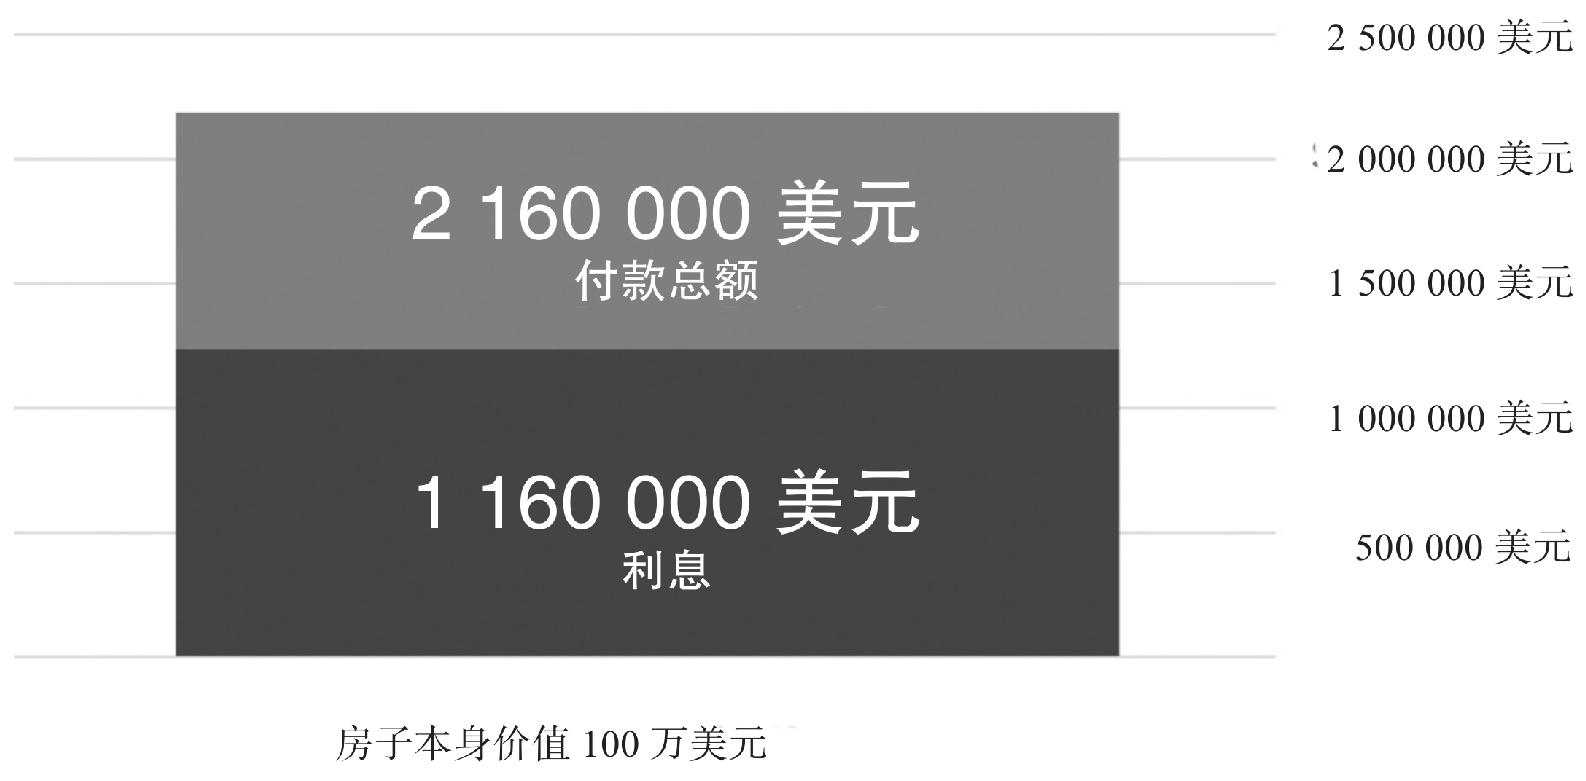
\includegraphics[width=0.84\linewidth,keepaspectratio]{image/17-1.jpg}
\caption{}\label{fig:17-1}
\end{figure}

对于大多数人来说，他们的抵押贷款是最大单笔的支出，但你并不知道，你每个月还的房贷，大部分都是还利息了。你要是知道，平均而言，每个美国人房贷加信用卡贷款和汽车贷款，34.5\%的税后工资都得拿去付利息了。我敢打赌，你看后并不会大吃一惊。这只是平均水平，很多人花在利息上的钱大大超过了自己收入的1/3。

那么你如何能够大幅削减那些巨大的利息支出呢？你如何减少你长期积累的利息支出——把那些钱拿回来，就能增加你争取财务自由的基金呢？答案非常简单，也可能会让你感到吃惊。

要是你借的是传统的固定利率的房贷，你只需要做一件事就行了，就是在贷款期间提前归还本金。这个月提前归还你下个月分摊的贷款本金，你就可以将原来30年的房贷在15年内还清本息，在大多数情况下这都行得通！这是不是意味着你每个月的月供要翻倍？根本不用！

\textbf{金钱威力法则3：}把你的房贷还款总额减掉一半！下个月你还了当月的房贷后，再拿出一些钱提前还掉本金——只是下个月房贷里的本金部分，不是全部本金，别害怕。

反正这些钱，都是你下个月肯定要付的钱，为什么不从你的口袋里提前一两个星期拿出来，这样以后你能给自己省下来一大笔钱。整体来看，你早期的房贷还款中有80\%\textasciitilde{}90\%，有些情况下可能会更多，都是去付利息了。平均而言，大多数美国人要么是还不起房贷了，只好断供，房子不要了，要么是过了五六年再融资，借新债还老债（这样又开始了新一轮新房贷还款，绝大部分是还利息的愚蠢做法）。

“太可惜了。”抵押贷款专家马克·爱森逊写了一本书《银行家的秘密》。他接受《纽约时报》采访时说：“有好几百万人，老老实实地每个月还房贷，因为他们不明白提前一个月还掉下个月的本金，只是多花了一点儿小钱，但能给自己带来巨大的好处。”

我们来看一个案例（详见以下表格）。平均每个美国家庭的房子价值27万美元，但是这个策略，不管你买房花了50万美元还是200万美元，都有效。要是你的贷款期限是30年，买的房子的价值属于美国平均水平——27万美元，每年的贷款利率是6\%，这需要你一开始每个月还房贷1618美元。用了这个方法，你要再拿出来270美元——这是下个月要还的房贷里的本金部分——其实是很少一笔钱，相当于你每个月房贷的1/6。你这个月多还的这270美元是本金，以后你永远不用为这笔本金付利息了。说得清楚些，你再也不用额外花钱付利息了，你只是在这个月还房贷的时候提前还了下个月的本金而已。

一直坚持用这种提前一个月归还本金的策略，你只用15年就能还完一个原来还款期限是30年的房贷。为什么不提前一个月还下个月的本金270美元？这样你就能把你的房贷还款年数缩短一半呢！如果你购买你的房子花了100万美元，那么你就可以省下50万美元，让它重新回到你的口袋里！一下子多出来相当于你半套房子的钱，这是不是会大大加快你通向财务自由的旅程？

% 来源：OEBPS/Text/Section0001_split_003.xhtml → image_10eeea85b3a6472886201323b214ab67.jpg
\begin{longtable}{@{}C{\dimexpr 0.12000\linewidth-1.60000\tabcolsep\relax}C{\dimexpr 0.21000\linewidth-1.60000\tabcolsep\relax}C{\dimexpr 0.21000\linewidth-1.60000\tabcolsep\relax}C{\dimexpr 0.21000\linewidth-1.60000\tabcolsep\relax}C{\dimexpr 0.25000\linewidth-1.60000\tabcolsep\relax}@{}}
\caption{美国房子的平均价格}\label{tab:17-1}\\
\toprule\noalign{\vskip 3pt}
{\heiti 月份} & {\heiti 付款} & {\heiti 本金} & {\heiti 利息} & {\heiti 余额} \\
\midrule
\endfirsthead
\multicolumn{5}{r}{续表}\\[0.6em]
\toprule\noalign{\vskip 3pt}
{\heiti 月份} & {\heiti 付款} & {\heiti 本金} & {\heiti 利息} & {\heiti 余额} \\
\midrule
\endhead
\bottomrule
\endfoot
\bottomrule
\multicolumn{5}{@{}p{\linewidth}@{}}{\footnotesize 单位：美元。}\\
\endlastfoot
1月 & 1\,618.79 & 268.79 & 1\,350.00 & 269\,731.21 \\
2月 & 1\,618.79 & 270.13 & 1\,348.66 & 269\,461.08 \\
3月 & 1\,618.79 & 271.48 & 1\,347.31 & 269\,189.60 \\
4月 & 1\,618.79 & 272.84 & 1\,345.95 & 268\,916.76 \\
\end{longtable}


\subsection{孩子，你可以开我的车}

并不只是房子能让我们省下一大笔钱。我有个儿子，非常喜爱宝马车，就是想要买一辆宝马车。在盼了很多年“终极驾驶神器”后，最终他分期付款买了一辆全新的、豪华配置的宝马车，他想要的功能这辆车全都具备了。买了这辆车后，他兴奋了好久。他爱这辆车开起来的那种感觉；他爱这辆车的马达轰鸣声，像是在对他甜言蜜语；他爱这辆车让他感觉很有面子。开宝马车的人，一看就知道很骄傲，很有抱负；开什么样的车，代表你是什么样的人，人就是车，车就是人——至少他是这样想的。

有好处必然也有坏处。宝马车好，价钱也高，花掉了他一大笔钱！他每个月还车贷的钱，本来可以用来还房贷。再过一两年，这辆车就会变得有些旧了，毫不奇怪，它会失去一些魅力。等到他30岁刚刚订婚后，他想去买一套房子给自己和未来的妻子住。结果一算账，他开始后悔了。他那辆宝马X6（双涡轮增压V8），每个月1200美元的车贷足够支付一套房子的房贷。

他也认识到了自己不再需要像原来那样开一辆豪车来显摆自己了。车，只不过是个交通工具而已。他明白了自己也可以开一辆大众帕萨特或者迷你库柏，那样也许更好、更新、更省油。

除此之外，原来开宝马车给他带来的快乐大部分都没有了。他在别的地方找到了快乐：买个房子，和他心爱的女人安个家，开始新的生活。不开宝马车，不再是牺牲自己了，相反，它变成了一个深思熟虑后的决定：把钱花在别的地方，开始为自己和家人打造一个财务上很安全的未来。

现在你如果是个汽车发烧友，非常喜欢车（像我一样），那我不是要告诉你去开一辆大众汽车。对于很多人来说，法拉利、保时捷，还有新出来的特斯拉，简直无法让人抗拒。如果你的计划已经完成了，你的财富积累达到了你想要达到的财务目标，不管怎么样，你想开什么车就开什么车吧。但是如果你的财富积累还没有达到你的财务计划目标，或者你现在奔向财务目标的财富积累速度还不够快，那么也许是时候重新思考一下，你现在开这样的豪车值不值，看看你能不能找到省下不少钱的办法，把更多的钱加入你的财务自由基金里。

还记得安吉拉吗？她读了本书的初稿后，就去买了辆新车——这是他人生买的第一辆全新的车子！我们来看看安吉拉买新车时算的账：他可以把旧车卖掉，每个月省下来400美元的修车费，一年就能省下来接近5000美元，把这些钱储蓄起来做投资，就能开始利用复利增长。

\subsection{你还能做些什么来省一大笔钱？}

并不是只有房子和车子这两个地方，能让我们省出一大笔钱。还有哪些地方的支出已经不能给你带来价值了？我知道，节衣缩食、紧紧巴巴、抠抠搜搜地过日子，对于大多数人来说没有吸引力。我可不想完全按照预算来花钱，我想你也不喜欢。但是我相信，确实需要制订一个花钱的计划。我喜欢计划这个做法，看看怎么花钱能给我带来最大的幸福和快乐，同时也能保证我长期努力之后实现财务自由。

不过，公平地说，你如果也是那种人，会抱怨地说：“去你的吧，我才不会想办法省钱呢，我只想专注于赚钱，赚得更多就行了。”那么你可以直接跳过这一章，直接翻到下一章，看一看怎么赚得更多和增加更多的价值。如果省钱的想法听起来让你筋疲力尽，或者你一听省钱就心烦，这也没关系，你还有其他四个策略能帮助你加快财富积累速度，我不希望你会错过另外加快财富积累的四招，不要只是因为省钱这一招不是你喜欢的，就连其他的四招也不看了。但是你如果确实愿意学些简单有效的省钱妙招，就接着读下去。我敢保证，你只要做几件小事情，长期就会产生重大的影响——让你长期能够积累一笔巨大的财富。

公平地说，亚马逊网上书店和那些实体书店里面有很多书教你如何省下更多的钱。戴夫·拉姆齐是一个非常有心的男人，他写了好几本书教大家如何省钱。苏茜·欧曼女士也写了好几本书教你省钱。这些书都值得一读。但是，我们还是会用几页的简短篇幅，重点介绍几个实用的、简单的省钱策略。

有一件事确定无疑是值得去做的，你可以列一个开支计划来帮助你提前决定怎么花你的钱，把你的钱花到哪里，以给你今天和未来带来最大的回报。

还记得在第3章中，我们看到一个省钱的实际生活案例，订购比萨外卖在家里和朋友们聚餐，而不是出去到饭店吃晚饭，这样做每个星期能给你省下40美元，一年就能省2080美元。那么按照8\%的年收益率计算，再过40年这笔钱就会变成50万美元以上，这可是100万美元的一半！它能让你过上幸福的退休生活，远远胜过现在大多数美国人的退休生活，他们的退休金可没有这么多。这种小钱用来投资，或者把它放到我们的退休金账户做投资，竟然会利滚利地增长到50万美元，这肯定会让我们重新思考，每天早上花钱喝一大杯咖啡究竟值不值。

财务专家戴维·巴赫是我的好朋友，他自己创业，就是从参加了我的财务研讨会开始的，那是20多年前的事了。他决定要追寻他的梦想，帮助人们实现财务独立。过了几年之后，我高薪聘请他第一次发表付费演讲。现在，他用激情和奉献帮助教育美国人学习投资理财知识，他写的畅销书《自动成为百万富翁》卖出了400多万册。这本书的核心讲的其实就是一句话：省小钱发大财。他说的小钱，最典型的代表就是很多美国人早上必须喝一杯拿铁咖啡，他在书里称之为“拿铁因子”。其实他说的不仅是拿铁咖啡，也包括所有你不经意间花的小钱。这些小钱加在一起其实会消耗掉我们很大一笔财富，而我们根本没有意识到。但是如果你很爱喝咖啡，那么你知道这个爱好会花掉你多少钱吗？假设你只是轻度上瘾，一天一杯而已，一天一杯也就4美元（换成人民币也就30元左右），但是日积月累，过上20年，按照6\%的利率计算，你实际上相当于喝掉了5.65万美元（相当于人民币40万元）。只是每天喝上一杯咖啡，你付出的代价竟然这么大！但是我们还是要面对现实，那些星巴克的忠实粉丝可不是一天只去一次。爱喝咖啡的人一天会去两三次。一天一杯是一天4美元，一天两三杯就是一天十几美元，这样20年下来，按照6\%的利率计算，你相当于喝掉了141250美元（相当于100万元人民币）。这可够你的孩子在美国念四年大学的学费了！

如果你是个纯粹主义者呢？你才不会狂喝咖啡，摄入那么多咖啡因呢！你的身体是个圣殿，你十分小心地注意保健。但是瓶装水是你钟爱的东西。你也爱喝斐济或者依云矿泉水吗？公平地说，即使你只是到超市买几箱便宜的波兰矿泉水，你知道你每年花在瓶装水上的钱能有多少吗？我的一个年轻的女同事，我很敬重她，她也觉得自己很有社会责任感。她最近快要结婚了，未婚夫一无咖啡瘾，二无酒瘾，但是他喝矿泉水上瘾，会定期买上一箱12瓶、每瓶1.5升的矿泉水。天天喝那么多矿泉水，他这样做很聪明吗？他一次会买3箱，总共36瓶，够他喝上两个星期，这样要花掉他75美元。一个月去买两次，他在喝水上每个月就要花150美元，一年下来接近1800美元——他花这么多钱买的东西，可以打开水龙头随便喝，一分钱也不用花。讲究一些的，可以买个德国产的碧然德净水器，再买几个耐尔水壶，让你一样可以天天喝上非常干净的水，一年只要花50\textasciitilde{}60美元。别忘了，他这样天天喝瓶装矿泉水，既在毁掉我们的地球，又在毁掉自己的钱包。我想，我这个女同事的未婚夫要是每年能把花在喝瓶装水上的1800美元省下来，放到他们的储蓄账户中，利用复利不断增值，他们肯定会开心得多。因为每年1800美元，按照每年8\%的收益率计，过上40年，就会变成503605美元。但这些钱都给他喝水喝掉了！

我并不是说你必须放弃喝瓶装水，或者再也不喝咖啡了，但是和喝水、喝咖啡一样，确实有些小地方能让你省出来不少钱，现在找一找那些能给你省大钱的小地方。

最后一个省钱的地方是购物，特别是一时高兴冲动的购物：你知道的，就在那一刻，你非常喜爱那些名牌奢侈品，像很贵的包包，很漂亮的爱马仕领带，你觉得非买不可。丽莎是个年轻的妈妈，来自那什维尔，非常喜欢那些精美的东西。她一冲动就会买名牌奢侈品，这都快把她丈夫逼疯了。丽莎回到家里，经常不是身上穿着一件新裙子，就是脚上穿着一双非常亮丽的新鞋子，她的丈夫总是一成不变地问：“你这些东西是打折买的吗？”或者问：“你有没有到网上查查同样的衣服在哪里卖得更便宜呢？”两人吵了几次架，他们最终达成协议，决定实行一个新的计划。要是丽莎发现自己突然心血来潮来到纽约第五大道的萨克斯百货商店，或者进了周仰杰鞋店，又看上了一件衣服或者一双鞋子，非买不可，她要拍下来这个东西的照片，发给她丈夫。丽莎给丈夫两个星期的时间，到网上用更便宜的价格买下来，不然的话，丽莎就会打电话给实体店全价购买。不过丽莎像个小绵羊一样地害羞承认，不管她想要买的是什么，在超过80\%的情况下，她的丈夫都能在网上找到更便宜的价格——一般都能打八折，有时会低到七折。

你可以学学丽莎和她丈夫到网上查所有的购物返利计划，这能给你省下真金白银。一些网站能帮你从日常花费上返利，帮你攒学费，从网上购买、出去吃饭到外出旅游，都能帮你省钱。你可以把你省下来的这些钱用于还你的学生贷款，存进储蓄账户，或者529大学储蓄计划（这是一个能够递延纳税的储蓄计划，由父母设立来为孩子积攒大学学费）。如果孩子大学毕业了或者孩子上大学并不是最优先考虑的事，你也可以存下一笔现金。网上有几百个购物返利网站，都能给你节省10\%\textasciitilde{}30\%的费用。丽莎和她的丈夫把所有得到的购物返利都打进了他们的教育基金账户，现在每个人都对那双细高跟鞋感觉好多了。

当一天结束的时候，问自己这个问题：我的花费，不管是大还是小，给我带来的兴奋激动还和过去一样吗？这并不是要剥夺你的购物权利，而是要调整你的花钱习惯，花的钱要符合你的核心价值观，只在那些真正对你非常重要的体验上，放纵自己多花一些钱。精心考虑确有必要之后才会花钱来买，这种习惯能让你的钱花得值，能让你的生活品质持续保持下去，持续给你带来幸福和快乐。不管你现在的年纪多大，这辈子还有20年、30年、40年可以投资，不管你现在攒的钱是多是少，不管你每年能省多少钱，也不管你还有多少年继续省钱，你都可以利用复利无与伦比的巨大力量，省得更多，赚得更多。财务安全，财务独立，不管你的财务目标是什么，你实现目标的速度都会大大加快，因为你省下来不必要的花费，把这些钱储蓄起来做投资，用复利让你的财富积累得越来越快。

这里的关键不是生活方式，而是时机选择。为什么今天不做出一些简单的改变，每天省些小钱，日积月累，利用复利增值，使它们变成大钱，确保你有足够的财富，人生之路可以一路顺利地走下去，享受你想要的生活方式，实现你的梦想？你仍然可以享受生活中那些奢侈消费带来的快乐，但这是你主动控制，而不是你受冲动控制。你选择如何分配你的资金，投资到让你的钱花得最值的地方。有很多简单的省钱妙招，你可以从以前按照合同还房贷变成提前归还下个月的本金，也可以把原来开的豪华汽车换成经济实用型的汽车，也可以从实体店购买换成从网上购买。有很多省钱妙招，真的能给你省下真金白银，日积月累，每年省下来的钱的数字相当大，要是你能够找到这些省钱的地方，把省下来的钱做投资，利用复利的力量，几十年下来，你就能积累几万美元、几十万美元，甚至上百万美元的财富。

现在翻到下一章，我要告诉你一个大招，让你的计划实施的速度更快，获得财务独立的速度更快。那就是我所知道的加速财务积累的最快方式：赚得更多。

\subsection{多多留心，处处能省}

这里有个练习，只有6步，很简单，你能很快做完。它能帮助你深入思考省钱这件事——更加积极，更加自觉。

第1步：头脑风暴。快速回想所有一再重复发生的费用，你可以取消或者减少，以削减你的费用支出。比如，汽车保险、手机账单、午餐饭钱、电影票。想想有哪些重复性花费，你可以做些改变，多省些钱。

% 来源：OEBPS/Text/Section0001_split_003.xhtml → image_cf2b7e0e026e47908034505bffdf1c39.jpg
\begin{longtable}{@{}C{\dimexpr 0.12000\linewidth-1.71429\tabcolsep\relax}C{\dimexpr 0.12000\linewidth-1.71429\tabcolsep\relax}C{\dimexpr 0.13500\linewidth-1.71429\tabcolsep\relax}C{\dimexpr 0.14000\linewidth-1.71429\tabcolsep\relax}C{\dimexpr 0.15500\linewidth-1.71429\tabcolsep\relax}C{\dimexpr 0.15500\linewidth-1.71429\tabcolsep\relax}C{\dimexpr 0.17500\linewidth-1.71429\tabcolsep\relax}@{}}
\caption{开始投资越早，积累的财富越多}\label{tab:17-2}\\
\toprule\noalign{\vskip 3pt}
{\heiti 日常投资数} & {\heiti 每月投资数} & {\heiti 10年} & {\heiti 20年} & {\heiti 30年} & {\heiti 40年} & {\heiti 50年} \\
\midrule
\endfirsthead
\multicolumn{7}{r}{续表}\\[0.6em]
\toprule\noalign{\vskip 3pt}
{\heiti 日常投资数} & {\heiti 每月投资数} & {\heiti 10年} & {\heiti 20年} & {\heiti 30年} & {\heiti 40年} & {\heiti 50年} \\
\midrule
\endhead
\bottomrule
\endfoot
\bottomrule
\multicolumn{7}{@{}p{\linewidth}@{}}{\footnotesize 假设年投资收益率为10\%。单位：美元。}\\
\endlastfoot
5 & 150 & 30\,727 & 113\,905 & 339\,073 & 948\,612 & 2\,598\,659 \\
10 & 300 & 61\,453 & 227\,811 & 678\,146 & 1\,897\,224 & 5\,197\,317 \\
15 & 450 & 92\,180 & 341\,716 & 1\,017\,220 & 2\,845\,836 & 7\,795\,976 \\
20 & 600 & 122\,907 & 455\,621 & 1\,356\,293 & 3\,794\,448 & 10\,394\,634 \\
30 & 900 & 184\,360 & 683\,432 & 2\,034\,439 & 5\,691\,672 & 15\,591\,952 \\
40 & 1\,200 & 245\,814 & 911\,243 & 2\,712\,586 & 7\,588\,895 & 20\,789\,269 \\
50 & 1\,500 & 307\,267 & 1\,139\,053 & 3\,390\,732 & 9\,486\,119 & 25\,986\,586 \\
\end{longtable}


第2步：这些东西或者活动花掉你多少钱呢？重点标出这些花费中占比最大的那一项，记下来这项最大花费每次会用掉你多少钱。接下来再算一算你每个星期纵容自己做几次这种花费，对自己实话实说，不要只是想当然。

第3步：现在，用从0到10来衡量你的快乐程度（0代表根本没有快乐，10代表极端快乐），你从上面每个费用项目上得到的快乐有多少呢？给每个花钱的活动或者东西写上一个代表快乐程度的数字，帮助你把这些费用和你的实际生活联系到一起。

第4步：接下来想一想，如果拥有绝对的财务自由，你会有什么样的感觉。第15章提出了一个概念：你梦想的价码，即实现你的梦想需要的钱。你还记得你脑子里有什么反应吗？这让你有什么样的感觉？但是你要记住，这只是你体验到的抽象感觉，理论上的感觉。现在呢，你离梦想很近了，足以细细品尝一下。如果你实现了绝对财务自由，你会享受什么，拥有什么，做什么，成为什么样的人，给予什么呢？

第5步：决定什么对你更加重要，是你从上面列的费用清单中那些一再重复发生的费用中得到的快乐，还是得到绝对财务自由让你感觉到的快乐呢？记住，生活就是平衡，你不需要放弃你的费用清单上的每一样东西，什么东西也不买，什么钱都不花，去追求那种绝对财务自由的感觉。

第6步：至少写下来三项费用，是你下定决心要完全放弃的。计算一下，这会让你下一年省下来多少钱。

% 来源：OEBPS/Text/Section0001_split_003.xhtml → image_3d9a68ee8261413191f586eb722d2d94.jpg
\begin{longtable}{|C{\dimexpr 0.10000\linewidth-2\tabcolsep-0.4667pt\relax}|C{\dimexpr 0.18000\linewidth-2\tabcolsep-0.4667pt\relax}|C{\dimexpr 0.18000\linewidth-2\tabcolsep-0.4667pt\relax}|C{\dimexpr 0.17000\linewidth-2\tabcolsep-0.4667pt\relax}|C{\dimexpr 0.25000\linewidth-2\tabcolsep-0.4667pt\relax}|C{\dimexpr 0.12000\linewidth-2\tabcolsep-0.4667pt\relax}|}
\caption{控制花钱：快速练习自觉省钱}\label{tab:17-3}\\
\hline
{\heiti 序号} & {\heiti 项目/活动} & {\heiti 项目/活动支出} & {\heiti 每周的次数} & {\heiti 总开支（项目开支乘以周数）} & {\heiti 愉悦度} \\
\hline
\endfirsthead
\multicolumn{6}{r}{续表}\\[0.6em]
\hline
{\heiti 序号} & {\heiti 项目/活动} & {\heiti 项目/活动支出} & {\heiti 每周的次数} & {\heiti 总开支（项目开支乘以周数）} & {\heiti 愉悦度} \\
\hline
\endhead
\hline
\endfoot
\hline
\endlastfoot
\rule{0pt}{2.3em}1 &  &  &  &  &  \\
\hline
\rule{0pt}{2.3em}2 &  &  &  &  &  \\
\hline
\rule{0pt}{2.3em}3 &  &  &  &  &  \\
\hline
\rule{0pt}{2.3em}4 &  &  &  &  &  \\
\hline
\rule{0pt}{2.3em}5 &  &  &  &  &  \\
\hline
\rule{0pt}{2.3em}6 &  &  &  &  &  \\
\hline
\multicolumn{6}{|l|}{\rule{0pt}{2.3em}每周总金额}\\
\hline
\multicolumn{6}{|l|}{\rule{0pt}{2.3em}每年总金额}\\
\end{longtable}

